\chapter{Notes}\label{chap:Notes}

\section{Complexity of matrix multiply}\label{sec:Complexity of matrix multiply}

Assume $\mathbf{A}$ is $m\times n$ and $\mathbf{B}$ is $n\times p$.
The naive algorithm takes $O\left(mnp\right)$ time.


\section{Representation of matrix}\label{sec:Representation of matrix}

Row major, col major, stride


\paragraph{How to calculate dimension of convolutional layer}

\[ \left\lfloor \frac{n_h - k_h + p_h + s_h}{s_h} \right\rfloor \times \left\lfloor \frac{n_w - k_w + p_w + s_w}{s_w} \right\rfloor \]

In which  \(n_h\)  means height of input, \(k_h\) means height of filter, \(p_h\) means padding of height, \(s_h\) means stride of height. So as \(n_w\), \(k_w\), \(p_w\), \(s_w\).


\section{Training Tricks}\label{sec:Training Tricks}


\paragraph{Batch normalization}

\[
	\textrm{BN}\left(\bm{x}\right)  = \gamma  \odot \frac{\bm{x} - \hat{\bm \mu}_\mathcal{B}}{\hat{\bm \sigma}_\mathcal{B}} + \beta
\]

Batch normalization is a technique that drastically reduces this problem.
The solution is surprisingly simple.
During training, a batch normalization layer calculates the mean and standard deviation of each of its input channels across the batch and normalizes by subtracting the mean and dividing by the standard deviation.
There are then two learned parameters for each channel, the scale (gamma) and shift (beta)~\cref{fig:batch_normalization}.
The output is simply the normalized input, scaled by gamma and shifted by beta~\cite{foster2022generative}.


When it comes to prediction, we may only want to predict a single observation, so there is no batch over which to calculate the mean and standard deviation.
To get around this problem, during training a batch normalization layer also calculates the moving average of the mean and standard deviation of each channel and stores this value as part of the layer to use at test time~\cite{foster2022generative}.

How many parameters are contained within a batch normalization layer? For every channel in the preceding layer, two weights need to be learned: the scale (gamma) and shift (beta).
These are the trainable parameters.
The moving average and standard deviation also need to be calculated for each channel, but since they are derived from the data passing through the layer rather than trained through backpropagation, they are called nontrainable parameters.
In total, this gives four parameters for each channel in the preceding layer, where two are trainable and two are nontrainable~\cite{foster2022generative}.

\begin{figure}
	\begin{center} 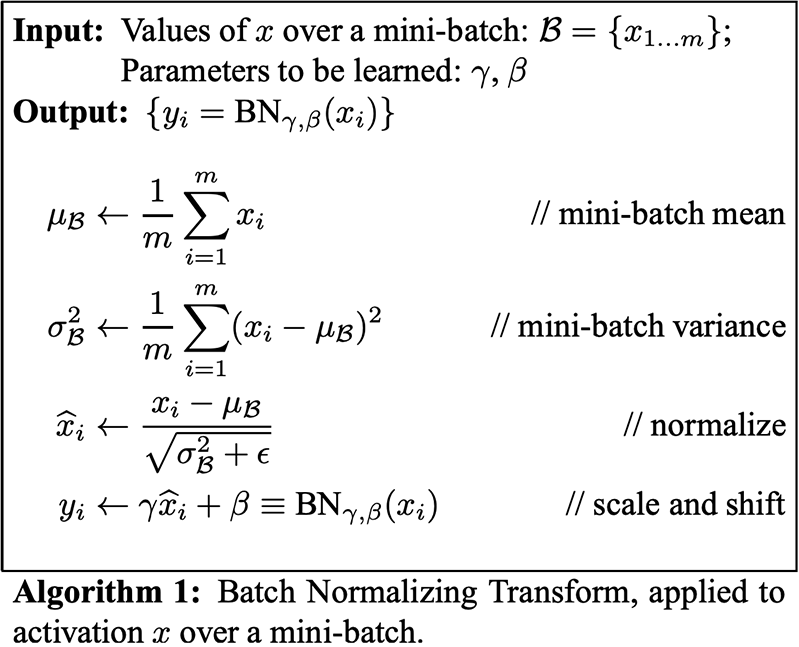
\includegraphics[width=0.95\textwidth]{figures/batch_normlization_page_76}
	\end{center}
	\caption{Batch Normalization}\label{fig:batch_normalization}
\end{figure}


\paragraph{Transposed Convolution}


Ignoring channels for now, let’s begin with the basic transposed convolution operation with stride of 1 and no padding.
Suppose that we are given a input tensor \( n_{h} \times n_{w} \) and a  kernel \( k_{h} \times  k_{w} \).
Sliding the kernel window with stride of 1 for \( n_{w} \) times in each row and \( n_{h} \) times in each column yields a total of \( n_{h}n_{w} \) intermediate results.
Each intermediate result is a \( \left(n_{h} + k_{h} -1\right) \times  \left(n_{w} + k_{w} - 1\right) \) tensor that are initialized as zeros.
To compute each intermediate tensor, each element in the input tensor is multiplied by the kernel so that the resulting tensor \( k_{h} \times k_{w} \) replaces a portion in each intermediate tensor.
Note that the position of the replaced portion in each intermediate tensor corresponds to the position of the element in the input tensor used for the computation.
In the end, all the intermediate results are summed over to produce the output~\cite[Chapter~14.10]{zhang2023dive}.


\begin{figure}
	\begin{center}
		\includesvg[width=0.95\textwidth]{figures/trans_conv}
	\end{center}
	\caption{Transposed Convolution~\cite[Chapter~14.10]{zhang2023dive}}\label{fig:trans_conv}
\end{figure}


Different from in the regular convolution where padding is applied to input, it is applied to output in the transposed convolution.
For example, when specifying the padding number on either side of the height and width as 1, the first and last rows and columns will be removed from the transposed convolution output.


\begin{figure}
	\begin{center}
		\includesvg[width=0.95\textwidth]{figures/trans_conv_stride2}
	\end{center}
	\caption{Transposed convolution with a kernel with stride of \( 2 \times 2 \). The shaded portions are a portion of an intermediate tensor as well as the input and kernel tensor elements used for the computation.~\cite{zhang2023dive}}\label{fig:trans_conv_stide}
\end{figure}


Consider implementing the convolution by multiplying matrices.
Given an input vector \( \mathbf{x} \) and a weight matrix \( \mathbf{W} \), the forward propagation function of the convolution can be implemented by multiplying its input with the weight matrix and outputting a vector \( y = \mathbf{W}\mathbf{x} \).
Since backpropagation follows the chain rule and \( \nabla_{x}\mathbf{y} = \mathbf{W}^{\top}\), the backpropagation function of the convolution can be implemented by multiplying its input with the transposed weight matrix \( \mathbf{W}^{\top}\) .
Therefore, the transposed convolutional layer can just exchange the forward propagation function and the backpropagation function of the convolutional layer: its forward propagation and backpropagation functions multiply their input vector with \( \mathbf{W}^{\top}  \) and \( \mathbf{W} \), respectively~\cite{zhang2023dive}.


